% Options for packages loaded elsewhere
\PassOptionsToPackage{unicode}{hyperref}
\PassOptionsToPackage{hyphens}{url}
%
\documentclass[
  12pt,
]{article}
\usepackage{amsmath,amssymb}
\usepackage{iftex}
\ifPDFTeX
  \usepackage[T1]{fontenc}
  \usepackage[utf8]{inputenc}
  \usepackage{textcomp} % provide euro and other symbols
\else % if luatex or xetex
  \usepackage{unicode-math} % this also loads fontspec
  \defaultfontfeatures{Scale=MatchLowercase}
  \defaultfontfeatures[\rmfamily]{Ligatures=TeX,Scale=1}
\fi
\usepackage{lmodern}
\ifPDFTeX\else
  % xetex/luatex font selection
\fi
% Use upquote if available, for straight quotes in verbatim environments
\IfFileExists{upquote.sty}{\usepackage{upquote}}{}
\IfFileExists{microtype.sty}{% use microtype if available
  \usepackage[]{microtype}
  \UseMicrotypeSet[protrusion]{basicmath} % disable protrusion for tt fonts
}{}
\makeatletter
\@ifundefined{KOMAClassName}{% if non-KOMA class
  \IfFileExists{parskip.sty}{%
    \usepackage{parskip}
  }{% else
    \setlength{\parindent}{0pt}
    \setlength{\parskip}{6pt plus 2pt minus 1pt}}
}{% if KOMA class
  \KOMAoptions{parskip=half}}
\makeatother
\usepackage{xcolor}
\usepackage[margin=1in]{geometry}
\usepackage{graphicx}
\makeatletter
\def\maxwidth{\ifdim\Gin@nat@width>\linewidth\linewidth\else\Gin@nat@width\fi}
\def\maxheight{\ifdim\Gin@nat@height>\textheight\textheight\else\Gin@nat@height\fi}
\makeatother
% Scale images if necessary, so that they will not overflow the page
% margins by default, and it is still possible to overwrite the defaults
% using explicit options in \includegraphics[width, height, ...]{}
\setkeys{Gin}{width=\maxwidth,height=\maxheight,keepaspectratio}
% Set default figure placement to htbp
\makeatletter
\def\fps@figure{htbp}
\makeatother
\setlength{\emergencystretch}{3em} % prevent overfull lines
\providecommand{\tightlist}{%
  \setlength{\itemsep}{0pt}\setlength{\parskip}{0pt}}
\setcounter{secnumdepth}{5}
\usepackage{url}
\usepackage{setspace}
%\singlespacing
%\onehalfspacing
%\doublespacing
\usepackage{lineno}
%\linenumbers
\usepackage[belowskip=0pt,aboveskip=0pt]{caption}
\usepackage{relsize}
\newcommand{\Fmsy}{\ensuremath{F_{\text{MSY}}}\xspace}
\newcommand{\Fspr}[1]{\ensuremath{F_{\text{{#1}\%}}}\xspace}
\newcommand{\afrb}{Alaska Fishery Research Bulletin\xspace}
\newcommand{\ajms}{African Journal of Marine Science\xspace}
\newcommand{\amb}{Advances in Marine Biology\xspace}
\newcommand{\bms}{Bulletin of Marine Science\xspace}
\newcommand{\bjssf}{Bulletin of the Japanese Society of Scientific Fisheries\xspace}
\newcommand{\cb}{Conservation Biology\xspace}
\newcommand{\cjfas}{Canadian Journal of Fisheries and Aquatic Sciences\xspace}
\newcommand{\ea}{Ecological Applications\xspace}
\newcommand{\eer}{Evolutionary Ecology Research\xspace}
\newcommand{\elet}{Ecology Letters\xspace}
\newcommand{\emod}{Ecological Modelling\xspace}
\newcommand{\ebf}{Environmental Biology of Fishes\xspace}
\newcommand{\ff}{Fish and Fisheries\xspace}
\newcommand{\fo}{Fisheries Oceanography\xspace}
\newcommand{\fr}{Fisheries Research\xspace}
\newcommand{\fb}{Fishery Bulletin\xspace}
\newcommand{\ijms}{ICES Journal of Marine Science\xspace}
\newcommand{\iccat}{Collective Volume of Scientific Papers ICCAT\xspace}
\newcommand{\jae}{Journal of Animal Ecology\xspace}
\newcommand{\jai}{Journal of Applied Ichthyology\xspace}
\newcommand{\jdc}{Journal Du Conseil International Pour L'exploration De La Mer\xspace}
\newcommand{\jdcp}{Journal Du Conseil Permanent International Pour L'exploration De La Mer\xspace}
\newcommand{\jembe}{Journal of Experimental Marine Biology and Ecology\xspace}
\newcommand{\jfb}{Journal of Fish Biology\xspace}
\newcommand{\jsr}{Journal of Sea Research\xspace}
\newcommand{\jtb}{Journal of Theoretical Biology\xspace}
\newcommand{\jfrbc}{Journal of the Fisheries Research Board of Canada\xspace}
\newcommand{\jnwafs}{Journal of Northwest Atlantic Fisheries Science\xspace}
\newcommand{\mcf}{Marine and Coastal Fisheries: Dynamics, Management, and Ecosystem Science\xspace}
\newcommand{\mb}{Marine Biology\xspace}
\newcommand{\meps}{Marine Ecology Progress Series\xspace}
\newcommand{\mfr}{Marine Fisheries Review\xspace}
\newcommand{\mpb}{Marine Pollution Bulletin\xspace}
\newcommand{\najfm}{North American Journal of Fisheries Management\xspace}
\newcommand{\nzjmfr}{New Zealand Journal of Marine and Freshwater Research\xspace}
\newcommand{\pnas}{Proceedings of the National Academy of Sciences USA\xspace}
\newcommand{\rpvrciemm}{Rapports et Proc\`es-Verbaux des R\'eunions. Conseil Internationale pour l'Exploration de la Mer\xspace}
\newcommand{\rpvrcpiemm}{Rapports et Proc\`es-Verbaux des R\'eunions. Conseil Permanent Internationale pour l'Exploration de la Mer\xspace}
\newcommand{\rfbf}{Reviews in Fish Biology and Fisheries\xspace}
\newcommand{\sajms}{South African Journal of Marine Science\xspace}
\newcommand{\tafs}{Transactions of the American Fisheries Society\xspace}

\newcommand{\anzjs}{Australian \& New Zealand Journal of Statistics\xspace}
\newcommand{\as}{Applied Statistics\xspace}
\newcommand{\csda}{Computational Statistics \& Data Analysis\xspace}
\newcommand{\ees}{Environmental and Ecological Statistics\xspace}
\newcommand{\jas}{Journal of Applied Statistics\xspace}
\newcommand{\jabes}{Journal of Agricultural, Biological, and Environmental Statistics\xspace}
\newcommand{\jasa}{Journal of the American Statistical Association\xspace}
\newcommand{\jrssb}{Journal of the Royal Statistical Society. Series B\xspace}
\newcommand{\sm}{Statistics in Medicine}

\usepackage{float}
\usepackage{amsmath}
\usepackage{pdflscape}
\usepackage{hyperref}
\usepackage{xspace}
\usepackage{bm}
\usepackage{caption,graphics}
\usepackage{graphicx}
\usepackage{makecell}
\usepackage{lineno}
\linenumbers
\renewcommand\figurename{Fig.}
\renewcommand{\figureautorefname}{Fig.}
\renewcommand{\tableautorefname}{Table}
\captionsetup{labelsep=period, singlelinecheck=false}
\newcommand{\changesize}[1]{\fontsize{#1pt}{#1pt}\selectfont}
\renewcommand{\arraystretch}{1.5}
\renewcommand\theadfont{}
\usepackage{booktabs}
\usepackage{longtable}
\usepackage{array}
\usepackage{multirow}
\usepackage{wrapfig}
\usepackage{float}
\usepackage{colortbl}
\usepackage{pdflscape}
\usepackage{tabu}
\usepackage{threeparttable}
\usepackage{threeparttablex}
\usepackage[normalem]{ulem}
\usepackage{makecell}
\usepackage{xcolor}
\ifLuaTeX
  \usepackage{selnolig}  % disable illegal ligatures
\fi
\usepackage[]{natbib}
\bibliographystyle{cjfas2.bst}
\IfFileExists{bookmark.sty}{\usepackage{bookmark}}{\usepackage{hyperref}}
\IfFileExists{xurl.sty}{\usepackage{xurl}}{} % add URL line breaks if available
\urlstyle{same}
\hypersetup{
  pdftitle={Evaluating the impact of log-normal bias-correction on a state-space stock assessment model},
  pdfauthor={Chengxue Li\^{}\{1,2,3*\}; Jonathan J. Deroba\^{}1; Timothy J. Miller\^{}1; Christopher M. Legault\^{}1; Charles T. Perretti\^{}1},
  hidelinks,
  pdfcreator={LaTeX via pandoc}}

\title{Evaluating the impact of log-normal bias-correction on a
state-space stock assessment model}
\author{Chengxue Li\(^{1,2,3*}\) \and Jonathan J.
Deroba\(^1\) \and Timothy J. Miller\(^1\) \and Christopher M.
Legault\(^1\) \and Charles T. Perretti\(^1\)}
\date{}

\begin{document}
\maketitle

\(^1\) Northeast Fisheries Science Center, Woods Hole Laboratory, 166
Water Street, Woods Hole, MA 02543 USA

\(^2\) School of Marine and Atmospheric Sciences, Stony Brook
University, Stony Brook, NY 11794, USA

\(^3\) Saltwater Inc., 733 N Street, Anchorage, AK 99501 USA

\(^*\)Corresponding author:
\href{mailto:chengxue.li@noaa.gov}{\nolinkurl{chengxue.li@noaa.gov}}

\vspace{0.5cm}

\textbf{ORCID:}

Chengxue Li:
\href{https://orcid.org/0000-0001-7518-7234}{0000-0001-7518-7234}

Tim J. Miller:
\href{https://orcid.org/0000-0003-1411-1206}{0000-0003-1411-1206}

Christopher M. Legault:
\href{https://orcid.org/0000-0002-0328-1376}{0000-0002-0328-1376}

Charles T. Perretti:
\href{https://orcid.org/0000-0002-4316-3630}{0000-0002-4316-3630}

\pagebreak

\hypertarget{abstract}{%
\section*{Abstract}\label{abstract}}
\addcontentsline{toc}{section}{Abstract}

In state-space stock assessment models, recruitment and numbers-at-age
are typically modeled as log-normal random variables, with bias
correction applied to ensure that their mean matches the expected mean
of the random variable. However, it remains unclear whether estimation
error in variance parameters, which influence bias correction,
propagates to estimates of population quantities. We conducted
simulation-estimation experiments to evaluate the effects of bias
correction for log-normal random variables and observations. We found
that applying bias correction on observations had minimal impact on
estimated population quantities, whereas applying bias correction on the
process had a significant effect, because estimation error in variance
parameters created bias in population estimates. Specifically, when both
recruitment deviations and numbers-at-age transitions were treated as
random effects, substantial bias in estimated annual recruitments and
\(SSB\) was found when bias correction was excluded in the operating
model but applied in the estimation model. In contrast, not using bias
correction had limited negative effects. Thus, we recommend avoiding
bias correction for log-normal random variables in state-space models,
especially when multiple random-effects processes are modeled
simultaneously.

\textbf{Keywords}: state-space models, random effects, bias correction,
recruitment, numbers-at-age transitions

\pagebreak

\hypertarget{introduction}{%
\section{Introduction}\label{introduction}}

State-space population models include random and fixed effects, where
random effects represent random processes that are separable from
observation error. Random effects now have been widely used to model a
variety of process errors in state-space stock assessments
\citep{Nielsen2014, Cadigan2015, Stock2021}. Perhaps the most common
random effects used in the state-space assessment model are deviations
on recruitment and numbers-at-ages 2+ (\(NAA\)). Recruitment and \(NAA\)
random effects are typically assumed to be log-normally distributed
\citep{Stock2021}.

Error modeled as normally distributed in log-space (i.e., log-normally
distributed), implies that error is multiplicative in natural space.
Log-normal error will increase the expected value of the population
process in natural space, where that increase is related to the variance
of the log-normal distribution. In order to ensure that this increase
does not occur, one can adjust the mean of the log-normal distribution,
known as ``bias-correction'' \citep{Methot2011}. Although there is not
universal agreement on whether bias-correction should be applied, an
important open question is the extent to which bias-correction affects
the accuracy of important assessment outputs such as recruitment and
spawning stock biomass (\(SSB\)). Here, we aim to address that question.

Bias in derived population quantities can be exacerbated by the
nonlinear transformation (e.g., exponentiation) of a random variable
\citep{Thorson2016}. Whether applying a bias correction term is
sufficient to accurately recapture the true population quantities
remains an open question \citep{Deroba2016}. Methot and Taylor (2011)
claimed that population abundance is informed by observations, which are
never perfectly accurate and often exhibit inter-annual variability in
both quantity and quality. Ignoring this source of variability can
induce bias in the estimation of recruitment variability, mean
recruitment, and hence management quantities
\citep{Methot2011, Thorson2016}. An additional plug-in ``multiplier''
was proposed in maximum likelihood estimation to provide more accurate
recruitment estimates \citep{Methot2011, Thorson2016}. However, their
approach is not appropriate for state-space models. In their simulation
experiments, recruitment was treated as a penalized fixed effect and was
not integrated out of the likelihood for estimation. In addition, they
fixed the recruitment standard deviation (\(\sigma_{Rec}\)) to avoid
potential estimation error. In state-space models, however,
\(\sigma_{Rec}\) is estimated using the marginal maximum likelihood,
which can influence the utility of the log-normal adjustment and derived
population quantities.

In addition, evidence has indicated that when multiple processes are
treated as random effects in a state-space model, the process variation
may not be reliably partitioned for each process due to processes being
confounded with each other
\citep{Trijoulet2020, Li2024, Liljestrand2024}. Improperly estimated
process variance can induce inaccurate adjustment and subsequently bias
population quantities. Moreover, when bias correction is applied to
multiple random processes (e.g., recruitment and \(NAA\)), an
interaction among the parameters associated with these random processes
is introduced in the marginal maximum likelihood estimation. The impacts
of this interaction on derived quantities are not fully understood.

To understand the caveats of applying bias correction to log-normal
random variables, as well as observations, we designed a
simulation-estimation experiment based on three stocks {[}Georges Bank
(GB) yellowtail flounder: \emph{Limanda ferruginea}, Gulf of Maine (GoM)
haddock: \emph{Melanogrammus aeglefinus}, and Atlantic mackerel:
\emph{Scomber scombrus}{]}. We explored scenarios where either
recruitment only or both recruitment and \(NAA\) were treated as random
effects, with different autocorrelation structures (see Section 2.4 for
more details). Overall, the goal of this study is to provide guidance on
bias-correction of log-normal random effects and observations in
state-space assessment models.

\hypertarget{methods}{%
\section{Methods}\label{methods}}

\hypertarget{overview}{%
\subsection{Overview}\label{overview}}

The Woods Hole Assessment Model (WHAM) is a state-space assessment model
(\url{https://timjmiller.github.io/wham}) \citep{Stock2021}. WHAM can
incorporate varying population and fishery processes, including
recruitment, \(NAA\), natural mortality, fishing selectivity, and survey
catchability \citep{Stock2021}. WHAM is currently used to manage various
stocks in the US northeast region. Below, we describe the population
processes and observations where a log-normal distribution is assumed.

\hypertarget{population-numbers-at-age}{%
\subsection{Population numbers-at-age}\label{population-numbers-at-age}}

The transitions between numbers-at-age are described as:

\begin{equation}
\log(N_{a,y}) =
\begin{cases}
\mu_{Rec} + \epsilon_{1,y} & \text{when } a = 1 \\
\log(N_{a-1, y-1} e^{-Z_{a-1, y-1}}) + \epsilon_{a,y} & \text{when } 1 < a < A \\
\log(N_{A-1, y-1} e^{-Z_{A-1, y-1}} + N_{A, y-1} e^{-Z_{A, y-1}}) + \epsilon_{A,y} & \text{when } a = A
\end{cases}
\end{equation}

where \(N_{a,y}\) is the numbers-at-age \(a\) in year \(y\),
\(\mu_{Rec}\) is the mean recruitment on the log scale, \(Z_{a,y}\) is
the total mortality rate for age \(a\) in year \(y\) (the sum of fishing
mortality \(F_{a,y}\) and natural mortality \(M_{a,y}\)), \(A\) defines
the plus-group, and \(\epsilon\) is the process error term, with
\(\epsilon_{1,y}\) representing recruitment deviations and
\(\epsilon_{a,y}\) (for \(a>1\)) representing NAA deviations.

Recruitment and \(NAA\) random effects are assumed to be log-normally
distributed with bias correction, given as:

\begin{equation}
\epsilon_{a,y} \sim 
\begin{cases} 
\mathcal{N}\left(-\frac{\sigma_{Rec}^2}{2}, \sigma_{Rec}^2\right), & \text{if } a = 1 \\
\mathcal{N}\left(-\frac{\sigma_{NAA}^2}{2}, \sigma_{NAA}^2\right), & \text{if } a > 1
\end{cases}
\end{equation}

where \(\sigma_{Rec}\) represents the standard deviation for recruitment
and \(\sigma_{NAA}\) represents the shared standard deviation for all
other ages. \(\sigma^2/2\) is the bias correction term. If bias
correction is not used, the mean of random effects in log space becomes
zero instead of \(-\sigma^2/2\). Note that when random effects are
autocorrelated across years, the bias correction term becomes
\(-\sigma^2 / [2 \cdot (1 - \rho_y^2)]\) where \(\rho_{y}\) indicates
the first-order autocorrelation across years. For more details please
see Stock and Miller (2021).

For example, assuming that recruitment is random about some mean value,
when bias correction is not applied:

\begin{equation}
R_{y} = \bar{R}_{y} \cdot e^{\epsilon_{y}}, \text{ with } \epsilon_y \sim \mathcal{N}(0, \sigma_{Rec}^2)
\end{equation}

where \(R_{y}\) is recruitment in year \(y\), \(\bar{R}_{y}\) is the
mean recruitment estimated in the model, and \(\epsilon_{y}\) is the
inter-annual deviations from the mean recruitment in log space. The
expectation of the \(\bar{R}_{y} \cdot e^{\epsilon_{y}}\) in Eq. 3 is:

\begin{equation}
E[\bar{R}_{y} \cdot e^{\epsilon_{y}}] = E[\bar{R}_{y}] \cdot E[e^{\epsilon_{y}}] =
\bar{R}_{y} \cdot e^\frac{\sigma_{Rec}^2}{2}
\end{equation}

Then, because \(e^\frac{\sigma_{Rec}^2}{2} > 1\)

\begin{equation}
E[R_{y}] \neq \bar{R}_{y}
\end{equation}

Note that the median of \(e^{\epsilon_{y}}\) is 1 here, therefore
\(\bar{R}_{y}\) is ``median unbiased'', but \(\bar{R}_{y}\) is always
less than \(E[R_{y}]\) and the difference becomes larger as the variance
\(\sigma_{Rec}^2\) increases.

Therefore, a bias correction term can be applied here to ensure
\(E[R_{y}] = \bar{R}_{y}\):

\begin{equation}
R_{y} = \bar{R}_{y} \cdot e^{\left(\epsilon_{y} - \frac{\sigma_{Rec}^2}{2}\right)}, \text{ with } \epsilon_y \sim \mathcal{N}(0, \sigma_{Rec}^2)
\end{equation}

\hypertarget{aggregate-catch-and-indices}{%
\subsection{Aggregate catch and
indices}\label{aggregate-catch-and-indices}}

Observed, annual, aggregate fishery catch is also assumed to be
log-normally distributed:

\begin{equation}
\log(\hat{C}_{y}) \sim \mathcal{N} \left( \log(C_{y}) - \frac{\sigma^2_{C}}{2}, \sigma^2_{C} \right)
\end{equation}

where \(\hat{C}_{y}\) is the observed fleet catch in year \(y\),
\({C}_{y}\) is the unobserved true catch, \(\sigma^2_{C_{y}}\) is an
input variance for catch observation (fixed across years in our study),
and \(-\sigma^2_{C_{y}}/2\) is the bias correction term. Note that
\(-\sigma^2_{C_{y}}/2\) is omitted from the Eq. 7 when bias correction
is not applied. With bias correction, the observation model is specified
so that the mean equals the true catch (mean-unbiased); without bias
correction, the observation model is specified so that the median equals
the true catch (median-unbiased).

Observations of annual aggregate indices of abundance are handled
identically to the aggregate catch in Eq. 7.

\hypertarget{operating-model}{%
\subsection{Operating model}\label{operating-model}}

For each stock, operating models (OMs) were constructed by fitting to
real fishery and survey data and conditioning on parameter values
informed by recent stock assessments
\citep[e.g.,][]{nefsc2019haddock, nefsc2021mackerel, nefmc2023flounder}.
Within each random-effects structure (Tables S1--S3), we developed four
OM variants corresponding to different bias correction treatments: (1)
bias correction applied to both the random-effects process and
observations, (2) bias correction applied to observations only, (3) bias
correction applied to the random-effects process only, and (4) no bias
correction. Parameters for the random-effects processes in each OM are
provided in Tables S1--S3, and fishery and survey configurations are
summarized in \autoref{model_config_table}.

\hypertarget{simulationestimation-experiment}{%
\subsection{Simulation--estimation
experiment}\label{simulationestimation-experiment}}

The simulation experiment followed a full factorial design
(\autoref{OM_scenario_table}). For each OM variant, fixed-effect
parameters (including variance parameters for random effects) were used
to generate 100 realizations of recruitment and population dynamics.
Observation error was applied to produce 100 pseudo-datasets per OM.
These pseudo-datasets were then fitted with all four estimation model
(EM) variants differing in bias correction treatment, producing all
OM--EM bias correction combinations within the same random-effects
structure. This design produced both self-tests (EM bias correction
treatment matches OM bias correction treatment) and cross-tests (EM bias
correction treatment differs from OM bias correction treatment)
\citep{Deroba2015}. A model was considered converged if two criteria
were met: (1) the optimizer had successfully converged, and (2) the
Hessian matrix was invertible. Simulations in which any of the four EMs
failed to converge were discarded, and additional iterations were run
with new random seeds until 100 complete and converged simulation
replicates were obtained for every scenario.

\hypertarget{performance-metrics}{%
\subsection{Performance metrics}\label{performance-metrics}}

Model performance was evaluated by calculating the median relative error
of recruitment, \(NAA\), and \(SSB\) over the model years. The relative
error was calculated as:

\begin{equation}
\text{Relative Error}_{i} = \text{Median} \left( \frac{\hat{\theta}_{i,y}}{\theta_{i,y}} - 1 \right)
\end{equation}

where \(\theta_{i,y}\) represents the true value for year \(y\) from the
simulated pseudo-dataset \(i\), and \(\hat{\theta}_{i,y}\) is the
estimated value from the EM fitting to the pseudo-dataset. Then, the
median, 25th quantile, and 75th quantile of these psuedo-dataset medians
were calculated.

To provide a performance metric that incorporates both bias and variance
simultaneously, the root mean squared relative error (RMSR) was also
calculated:

\begin{equation}
\text{RMSR}_{i} = \sqrt{ \frac{1}{T} \sum_{y=1}^{T} \left( \frac{\hat{\theta}_{i,y} - \theta_{i,y}}{\theta_{i,y}} \right)^2 }
\end{equation}

where \(T\) is the total number of years in the simulation. The median,
25th quantile, and 75th quantile of these psuedo-dataset medians were
calculated.

Considering the asymmetric nature of relative error, which ranges from
-1 (100\% underestimation) to infinity (\(\infty\) overestimation), we
also calculated the symmetric signed percentage bias (SSPB) and median
log-quotient (MdLQ) to ensure that underestimation and overestimation
are penalized equally \citep{Morley2018}:

\begin{equation}
\text{SSPB}_{i} = 100 \times \text{sign}(\text{MdLQ}_{i}) \times \left( e^{|\text{MdLQ}_{i}|} - 1 \right)
\end{equation}

where

\begin{equation}
\text{MdLQ}_{i} = \text{median}\left( \log \left( \frac{\hat{\theta}_{i,y}}{\theta_{i,y}} \right) \right)
\end{equation}

Note that a value of zero for either SSPB or MdLQ indicates the model is
median-unbiased, while negative and positive values indicate
underestimation and overestimation, respectively.

Relative errors of mean recruitment (\(\mu_{Rec}\)), recruitment
standard deviation (\(\sigma_{Rec}\)), \(NAA\) standard deviation
(\(\sigma_{NAA}\)), and AR(1)-year autocorrelation (\(\rho_{y}\))
(hereafter referred to as random-effects parameters) were also
calculated for each pseudo-dataset \(i\):

\begin{equation}
\text{Relative Error}_{i} = \frac{\hat{\theta}_{i}}{\theta_{i}} - 1
\end{equation}

In addition, we used the Akaike Information Criterion (AIC) to evaluate
the best-fitting EM for each realization \(i\). To compare the relative
performance of the EM \(j\), we calculated the delta AIC (dAIC):

\begin{equation}
\Delta\text{AIC}_{i,j} = \text{AIC}_{i,j} - \min_{j}(\text{AIC}_{i,j})
\end{equation}

The proportions of EMs selected by AIC were also calculated to evaluate
AIC's ability to identify the correctly specified model.

\hypertarget{results}{%
\section{Results}\label{results}}

For OMs with only recruitment random effects, the patterns of self-tests
and cross-tests were similar, regardless of whether the autocorrelation
structure was IID or AR(1)-year. Similarly, in OMs with both recruitment
and \(NAA\) random effects, the performance differences between
self-tests and cross-tests were consistent across IID and AR(1)-year
autocorrelation structures (Figs. S1-S2). Given these consistent
patterns, the results from the IID and AR(1)-year OMs were combined for
simplicity, resulting in 200 simulation replicates for each random
effects structure. The effect of applying the bias correction to the
catch and survey observations was trivial relative to the bias
correction effect of the process errors. Therefore, to simplify the
analysis, we restricted both the OMs and EMs to two primary
configurations: one where bias correction was applied to both processes
and observations (hereafter `BC-ON'), and another where it was turned
off for both (hereafter `BC-OFF').

We found that convergence failures were often realization-specific
rather than model-specific. In most cases, if one EM failed to converge
for a given realization, all EMs failed for that same realization,
suggesting that convergence issues were driven by factors other than the
bias correction setting. Therefore, to better isolate the effect of bias
correction, we calculated a conditional convergence rate: the proportion
of simulations that converged for the misspecified model, given that the
correctly specified self-test had already converged. This provides a
clearer evaluation of how the bias correction mismatch impacts model
convergence, with results summarized across all stocks (Table S4).

All performance metrics considered (relative error, RMSR, MdLQ, and
SSPB) led to similar conclusions, for brevity, only the relative error
results are presented in the main text. The results for the other
metrics can be found in the supplementary materials (Figs. S4--S12).

\hypertarget{relative-error-of-recruitment}{%
\subsection{Relative error of
recruitment}\label{relative-error-of-recruitment}}

For OMs with only recruitment random effects, the relative error in
recruitment estimates was small across all test scenarios. However, when
the OM included both recruitment and \(NAA\) random effects, model
performance became highly sensitive to mismatches in how bias correction
was applied between the OM and EM.

Specifically, applying bias correction in the EM but not in the OM led
to substantial overestimation of recruitment (7-37\%), with the most
severe bias observed for GB yellowtail flounder (37\%), followed by
Atlantic mackerel (14\%) and GoM haddock (7\%). Conversely, applying
correction in the OM but not the EM resulted in only a slight
underestimation for Atlantic Mackerel (8\%), while estimates for the
other two stocks were relatively unbiased (\autoref{fig:Median_Rec}).
The poor performance in the former case was corroborated by a greater
magnitude of RMSR (Fig. S4), MdLQ (Fig. S7), and SSPB (Fig. S10).

\hypertarget{relative-error-of-ssb-and-naa}{%
\subsection{\texorpdfstring{Relative error of \(SSB\) and
\(NAA\)}{Relative error of SSB and NAA}}\label{relative-error-of-ssb-and-naa}}

Estimates of \(SSB\) were accurate when the OM included only recruitment
random effects. However, performance degraded in scenarios with both
recruitment and \(NAA\) random effects, particularly when there was a
mismatch in how bias correction was applied.

Specifically, applying bias correction in the EM but not the OM led to a
consistent overestimation of \(SSB\) (11\% for GB yellowtail flounder,
9\% for Atlantic mackerel, and 5\% for GoM haddock). Conversely,
applying correction in the OM but not the EM resulted in a smaller
underestimation, which was negligible for GB flounder and GoM haddock
(close to 0\%) and 7\% for Atlantic mackerel (\autoref{fig:Median_SSB}).
This large positive bias in the former case also translated into a
greater overall model error, such as RMSR (Fig. S5), MdLQ (Fig. S8), and
SSPB (Fig. S11). The same pattern of bias and overall error was mirrored
in the estimates of \(NAA\) (Fig. S3, Fig. S6, Fig. S9, Fig. S12).

\hypertarget{relative-error-of-random-effects-parameters}{%
\subsection{Relative error of random-effects
parameters}\label{relative-error-of-random-effects-parameters}}

Recruitment standard deviation was accurately estimated, or slightly
underestimated (\autoref{fig:Rec_sigma}). When both recruitment and
\(NAA\) were treated as random effects in the OM, a systematic
underestimation of \(NAA\) standard deviation was found across
self-tests and cross-tests, with the magnitude of underestimation
ranging between -30\% and -10\% (\autoref{fig:NAA_sigma}). Such
consistent underestimation was also found for the AR(1)-year
autocorrelation parameter (Fig. S13).

\hypertarget{aic}{%
\subsection{AIC}\label{aic}}

Although the correctly specified EM was generally preferred based on
AIC, the difference in AIC between the correct model and the
misspecified model was usually less than two units
(\autoref{fig:AIC_select}). Therefore, using the standard rule of thumb
that dAIC \textgreater{} 2 represents a significant difference in model
performance, AIC would most often not be useful for determining whether
bias correction should be applied or not.

\hypertarget{discussion}{%
\section{Discussion}\label{discussion}}

\hypertarget{log-normal-random-effects}{%
\subsection{Log-normal random effects}\label{log-normal-random-effects}}

Our results suggest that bias correction has minimal impact on the
estimation of recruitment and \(SSB\) in state-space models when only
recruitment random effects were present, as both quantities were
accurately estimated in self-tests and cross-tests. However, in models
with both recruitment and \(NAA\) random effects, mismatches in bias
correction between the EM and OM (e.g., EM with bias correction while OM
without, or vice versa) led to biases in both recruitment and \(SSB\)
estimates. Recruitment estimates were particularly sensitive, with a
maximum median error of 37\% overestimation when the EM included bias
correction but the OM did not, compared to a maximum median error of 8\%
underestimation in the opposite scenario. For \(SSB\), biases were
generally smaller but still notable, where excluding bias correction in
the EM led to less bias in cross-tests, compared to applying it. The
lower magnitude of relative error in \(SSB\) compared to recruitment in
cross-tests is likely due to the relatively smaller process variance in
\(NAA\). This reduced variance minimizes the contribution of bias
correction to \(NAA\) estimates when transformed back to the natural
scale, and subsequently to \(SSB\). In contrast, the high variability in
recruitment amplifies even small estimation biases in process variance,
leading to exponentially larger biases in recruitment estimates when
transformed back to the natural scale.

When bias correction is applied to a log-normal random variable,
accurately estimating the variance parameters associated with random
effects is crucial to ensure that the derived log-normal quantities are
correctly transformed back to values on the natural scale. Our study
demonstrated that, in most cases, recruitment standard deviation
(\(\sigma_{Rec}\)) was well estimated in EMs with bias correction,
resulting in accurate population quantity estimates when the OM included
only recruitment random effects. In general, with bias correction, both
the mean (\(\mu_{Rec}\)) and standard deviation (\(\sigma_{Rec}\)) of
recruitment jointly influence annual recruitment estimates. When only
recruitment deviations are treated as random effects, if
\(\sigma_{Rec}\) is slightly underestimated, \(\mu_{Rec}\) may also be
underestimated to compensate and maintain a desired solution. This
interaction partially explains why recruitment estimates in our study
remained relatively unbiased when bias correction was applied in the EM
but not in the OM, or vice versa. Additionally, when only recruitment
deviations are treated as random effects in the OM, the system becomes
simplified by confining the process error to a single source of
uncertainty. This allows process variation to be restrictively
controlled, even when there is a mismatch between the data generation
process (OM) and the fitting process (EM) regarding bias correction.
However, when random effects are applied to both recruitment and
\(NAA\), their interaction introduces additional complexity to the
model, raising estimation challenges in disentangling their individual
contributions to the data. This interaction effect, coupled with the
mismatch between the data generation process and the fitting process
with respect to bias correction, likely contributes to discrepancies in
the estimation of population quantities.

The variability of \(NAA\) process error (i.e., \(\sigma_{NAA}\)), which
contributes to bias correction, can be underestimated in state-space
models for several reasons. Simulation studies have shown that
estimation bias in variance parameters associated with random effects
often arises from multiple confounding processes interacting with one
another, regardless of the magnitude of process variation
\citep{Li2024,Liljestrand2024}. Furthermore, variances may not be
properly apportioned among different random-effects processes when one
process exhibits high variability. For instance, Liljestrand et
al.~(2024) found that when recruitment and selectivity displayed low
variability but survival (i.e., \(NAA\)) had high variability, some of
the survival variation in the estimation model was misallocated to
recruitment. Additionally, underestimation of process variance is common
in maximum likelihood estimation, where variance estimates tend to
shrink when the sample size is insufficient to fully capture the
variability of the process. We found significant correlations between
\(\sigma_{NAA}\) and \(\sigma_{Rec}\) in cross-tests with BC-ON in the
EM (Figs. S15-S16). Given that estimation error of key outputs appears
to be related to the level of \(\sigma_{NAA}\) (Fig. S17-S18), and that
the species with the highest \(\sigma_{NAA}\) also had the largest
estimation error in cross-tests (GB yellowtail flounder, Figs 1-2),
there appears to be a link between \(\sigma_{NAA}\) and estimation error
of key outputs. However, further research is needed to better understand
how exactly this error in \(\sigma_{NAA}\) and other parameters
propagates to error in recruitment and \(SSB\).

\hypertarget{log-normal-observations}{%
\subsection{Log-normal observations}\label{log-normal-observations}}

In our study, the bias correction for log-normally distributed
observations had a limited impact on derived population quantities, in
contrast to the correction for process random effects. This is likely
because the observation error variance for fleet catch was fixed at
known, low values (CVs \(\le\) 0.2), following the configuration used in
recent assessments for these stocks. Fixing the variance prevents it
from being confounded with the process variance during estimation but
may also limit the potential influence of the observation-level bias
correction.

Our findings appear to contrast with those of \citet{aldrin2020}, who
found that applying bias correction to catch data could improve model
performance. A key difference lies in the treatment of observation
error: in their state-space assessment model (SAM), the catch
observation error variance was freely estimated, a flexibility that can
make the bias correction more influential, whereas in our study, it was
fixed. Furthermore, because the observation error for fleet catch in our
study was low and fixed (and generally smaller than the error for the
survey indices), the model likely weighted the fleet catch data heavily.
As noted by \citet{aldrin2020}, survey index observation error is often
less influential as it can be partially absorbed by the estimation of
catchability (q). The high confidence placed on the catch data in our
models may therefore limit the practical benefit of applying an
observation-level bias correction. In addition, our exploratory work
indicated that higher observation variance can be misattributed to
process variance, a finding consistent with previous reports of variance
confounding by \citet{Fisch2023}.

We therefore suggest that future simulation studies investigate how the
utility of log-normal bias correction for observations is affected by
key factors, including: (1) the relative magnitudes of observation and
process error, and (2) whether the observation error variance is fixed
or freely estimated within the model.

\hypertarget{implications-and-future-research-recommendations}{%
\subsection{Implications and future research
recommendations}\label{implications-and-future-research-recommendations}}

Restricted maximum likelihood (REML) has been proposed as an improvement
over marginal maximum likelihood estimation, as it provides an unbiased
estimator for the variance of random effects. Unlike marginal maximum
likelihood, REML calculates the variance of random effects by
integrating the likelihood over both random effects and non-variance
fixed effects and has been successfully implemented within Stock
Synthesis \citep{Thorson2015}. The application of REML is sparking
growing interest in state-space modeling due to its potential to improve
variance estimation for random effects and enhance the accuracy of
management quantity estimates \citep{Maunder2019, Thorson2019}. However,
little attention has been given to REML estimation of process variance
when multiple confounding random-effects processes occur simultaneously,
warranting further exploration in the future.

Our preliminary results suggest that the magnitude of estimation bias in
population quantities in cross-tests was not related to the level of
recruitment variability but was influenced by the level of the
variability of \(NAA\) in the OM. For instance, misspecified EMs with
bias correction tended to overestimate recruitment, with the degree of
overestimation increasing exponentially as \(\sigma_{NAA}\) increased
from 0.1 to 0.6 (Fig. S17). In contrast, misspecified EMs without bias
correction tended to underestimate recruitment as \(\sigma_{NAA}\)
increased, though to a lesser extent (Fig. S17). Similar patterns were
also observed for \(SSB\) (Fig. S18). Further investigation is needed to
better understand the underlying mechanisms driving these patterns.

Studies have demonstrated that ignoring data availability can introduce
bias in the log-normal adjustment term and result in inaccurate
estimates of log-normal random variables, such as recruitment deviations
\citep{Methot2011, Thorson2016}. This is because individual recruitment
estimates (\(\hat{R}_{y}\)) are directly informed by the data, and
variations in data quantity and quality across years can introduce
additional uncertainty to the estimate of \(\sigma_{Rec}\). Our
preliminary analysis of estimates from the intermediate period (with
improved data quantity for estimating recruitment and \(NAA\)) showed
only marginal improvement (Figs. S19-S20). This suggests that data
quantity and quality are less influential than the estimation of
random-effects parameters in adjusting log-normal random variables and
deriving management quantities. Future research could explore how
accounting for variability in data availability in state-space
assessment models might improve estimates of recruitment and other
derived quantities.

Overall, bias correction in state-space models should be applied with
caution, as its benefits are uncertain when the extent of bias in
parameters associated with random effects and their propagation into
derived population quantities cannot be reliably quantified. In the
absence of strong evidence in support of bias correction, we recommend
excluding it, as it appears to have less downside risk in cases where
supporting evidence is ambiguous.

\hypertarget{acknowledgements}{%
\section{Acknowledgements}\label{acknowledgements}}

We acknowledge the support provided by Saltwater Inc.~for facilitating
Chengxue Li's contribution to this project.

\hypertarget{competing-interests-statement}{%
\section{Competing interests
statement}\label{competing-interests-statement}}

One co-author, Timothy J. Miller, serves as a Guest Editor for CJFAS for
this special issue.

\hypertarget{credit-authorship-contribution-statement}{%
\section{CRediT authorship contribution
statement}\label{credit-authorship-contribution-statement}}

\textbf{Chengxue Li:} Conceptualization, Methodology, Software, Writing
- original draft, Formal analysis, Visualization.\\
\textbf{Jonathan J. Deroba:} Conceptualization, Funding acquisition,
Supervision, Writing - review \& editing.\\
\textbf{Timothy J. Miller:} Conceptualization, Software, Writing -
review \& editing.\\
\textbf{Christopher M. Legault:} Conceptualization, Writing - review \&
editing.\\
\textbf{Charles T. Perretti:} Conceptualization, Writing - review \&
editing.

\hypertarget{funding-statement}{%
\section{Funding statement}\label{funding-statement}}

This work was funded by NOAA Fisheries Northeast Fisheries Science
Center.

\hypertarget{data-availability-statement}{%
\section{Data availability
statement}\label{data-availability-statement}}

The data and code underlying this article are available on
\url{https://github.com/lichengxue/Bias_Correction_Project}, and have
been archived at \href{https://doi.org/10.5281/zenodo.17253797}{DOI:
10.5281/zenodo.17253797}.

\hypertarget{tables}{%
\section{Tables}\label{tables}}

\begin{table}[H]
\centering
\caption{Model configuration for GB Yellowtail Flounder, GoM Haddock, and Atlantic Mackerel. Note: The age composition likelihoods are defined as follows. `Dirichlet-miss0' uses the Dirichlet distribution where zero observations are treated as missing. `Logistic-normal-miss0' uses the logistic-normal distribution, also treating zeros as missing. `Logistic-normal-ar1-miss0' extends the logistic-normal model with a first-order autoregressive (AR1) error structure to account for temporal correlation.}
\label{model_config_table}
\begin{scriptsize} 
\begin{tabular}{p{4cm} p{3.5cm} p{3.5cm} p{3.5cm}} % Adjust column widths
\toprule
\textbf{Parameter} & \textbf{Flounder} & \textbf{Haddock} & \textbf{Mackerel} \\
\midrule
\textbf{Fleet Catch} & & & \\
\textbf{Period} & 1973-2022 & 1977-2018 & 1968-2019 \\
\textbf{Selectivity form} & Logistic & Age-specific & Age-specific \\
\textbf{Age comp. likelihood} & Dirichlet-miss0 & Logistic-normal-miss0 & Logistic-normal-ar1-miss0 \\
 & & & \\
\textbf{Survey Indices} & & & \\
\textbf{Period} & 1. 1973-2022 & 1. 1977-2018 & 1. 1979-2019 \\
 & 2. 1973-2022 & 2. 1977-2018 & 2. 2009-2019 \\
 & 3. 1987-2022 & & 3. 1974-2008 \\
\textbf{Selectivity form} & Logistic & Age-specific & Age-specific \\
\textbf{Age comp. likelihood} & Dirichlet-miss0 & Logistic-normal-miss0 & Logistic-normal-ar1-miss0 \\
\bottomrule
\end{tabular}
\end{scriptsize}
\end{table}


\begin{table}[H]
\centering
\caption{Summary of operating models (OMs) and estimation models (EMs) with different random-effects structures and bias correction scenarios. Each OM includes four bias correction scenarios (ON or OFF for process and observation, respectively).  Note that a shared AR(1)-year autocorrelation parameter ($\rho_y$) is used for both recruitment and $NAA$ random effects.}
\label{OM_scenario_table}
\begin{scriptsize} % Adjust the font size to scriptsize
\begin{tabular}{p{3cm} p{3cm} p{3.5cm} p{3.5cm}} % Adjusted column widths
\toprule
\textbf{Random Effects Structure} & \textbf{Parameters} & \textbf{Bias-Correct (Proc.)} & \textbf{Bias-Correct (Obs.)} \\
\midrule
\textbf{Rec (IID)} & $\sigma_{Rec}$ & ON & ON \\
                         &                                          & OFF & ON \\
                         &                                          & ON  & OFF \\
                         &                                          & OFF & OFF \\
\midrule
\textbf{Rec (AR1\(_y\))} & $\sigma_{Rec}, \rho_y$ & ON & ON \\
                         &                                          & OFF & ON \\
                         &                                          & ON  & OFF \\
                         &                                          & OFF & OFF \\
\midrule
\textbf{Rec+NAA (IID)} & $\sigma_{Rec}, \sigma_{NAA}$ & ON & ON \\
                         &                                          & OFF & ON \\
                         &                                          & ON  & OFF \\
                         &                                          & OFF & OFF \\
\midrule
\textbf{Rec+NAA (AR1\(_y\))} & $\sigma_{Rec}, \sigma_{NAA}, \rho_y$ & ON & ON \\
                         &                                          & OFF & ON \\
                         &                                          & ON  & OFF \\
                         &                                          & OFF & OFF \\
\bottomrule
\end{tabular}
\end{scriptsize}
\end{table}


\hypertarget{figures}{%
\section{Figures}\label{figures}}

\begin{figure}[H]
\centering
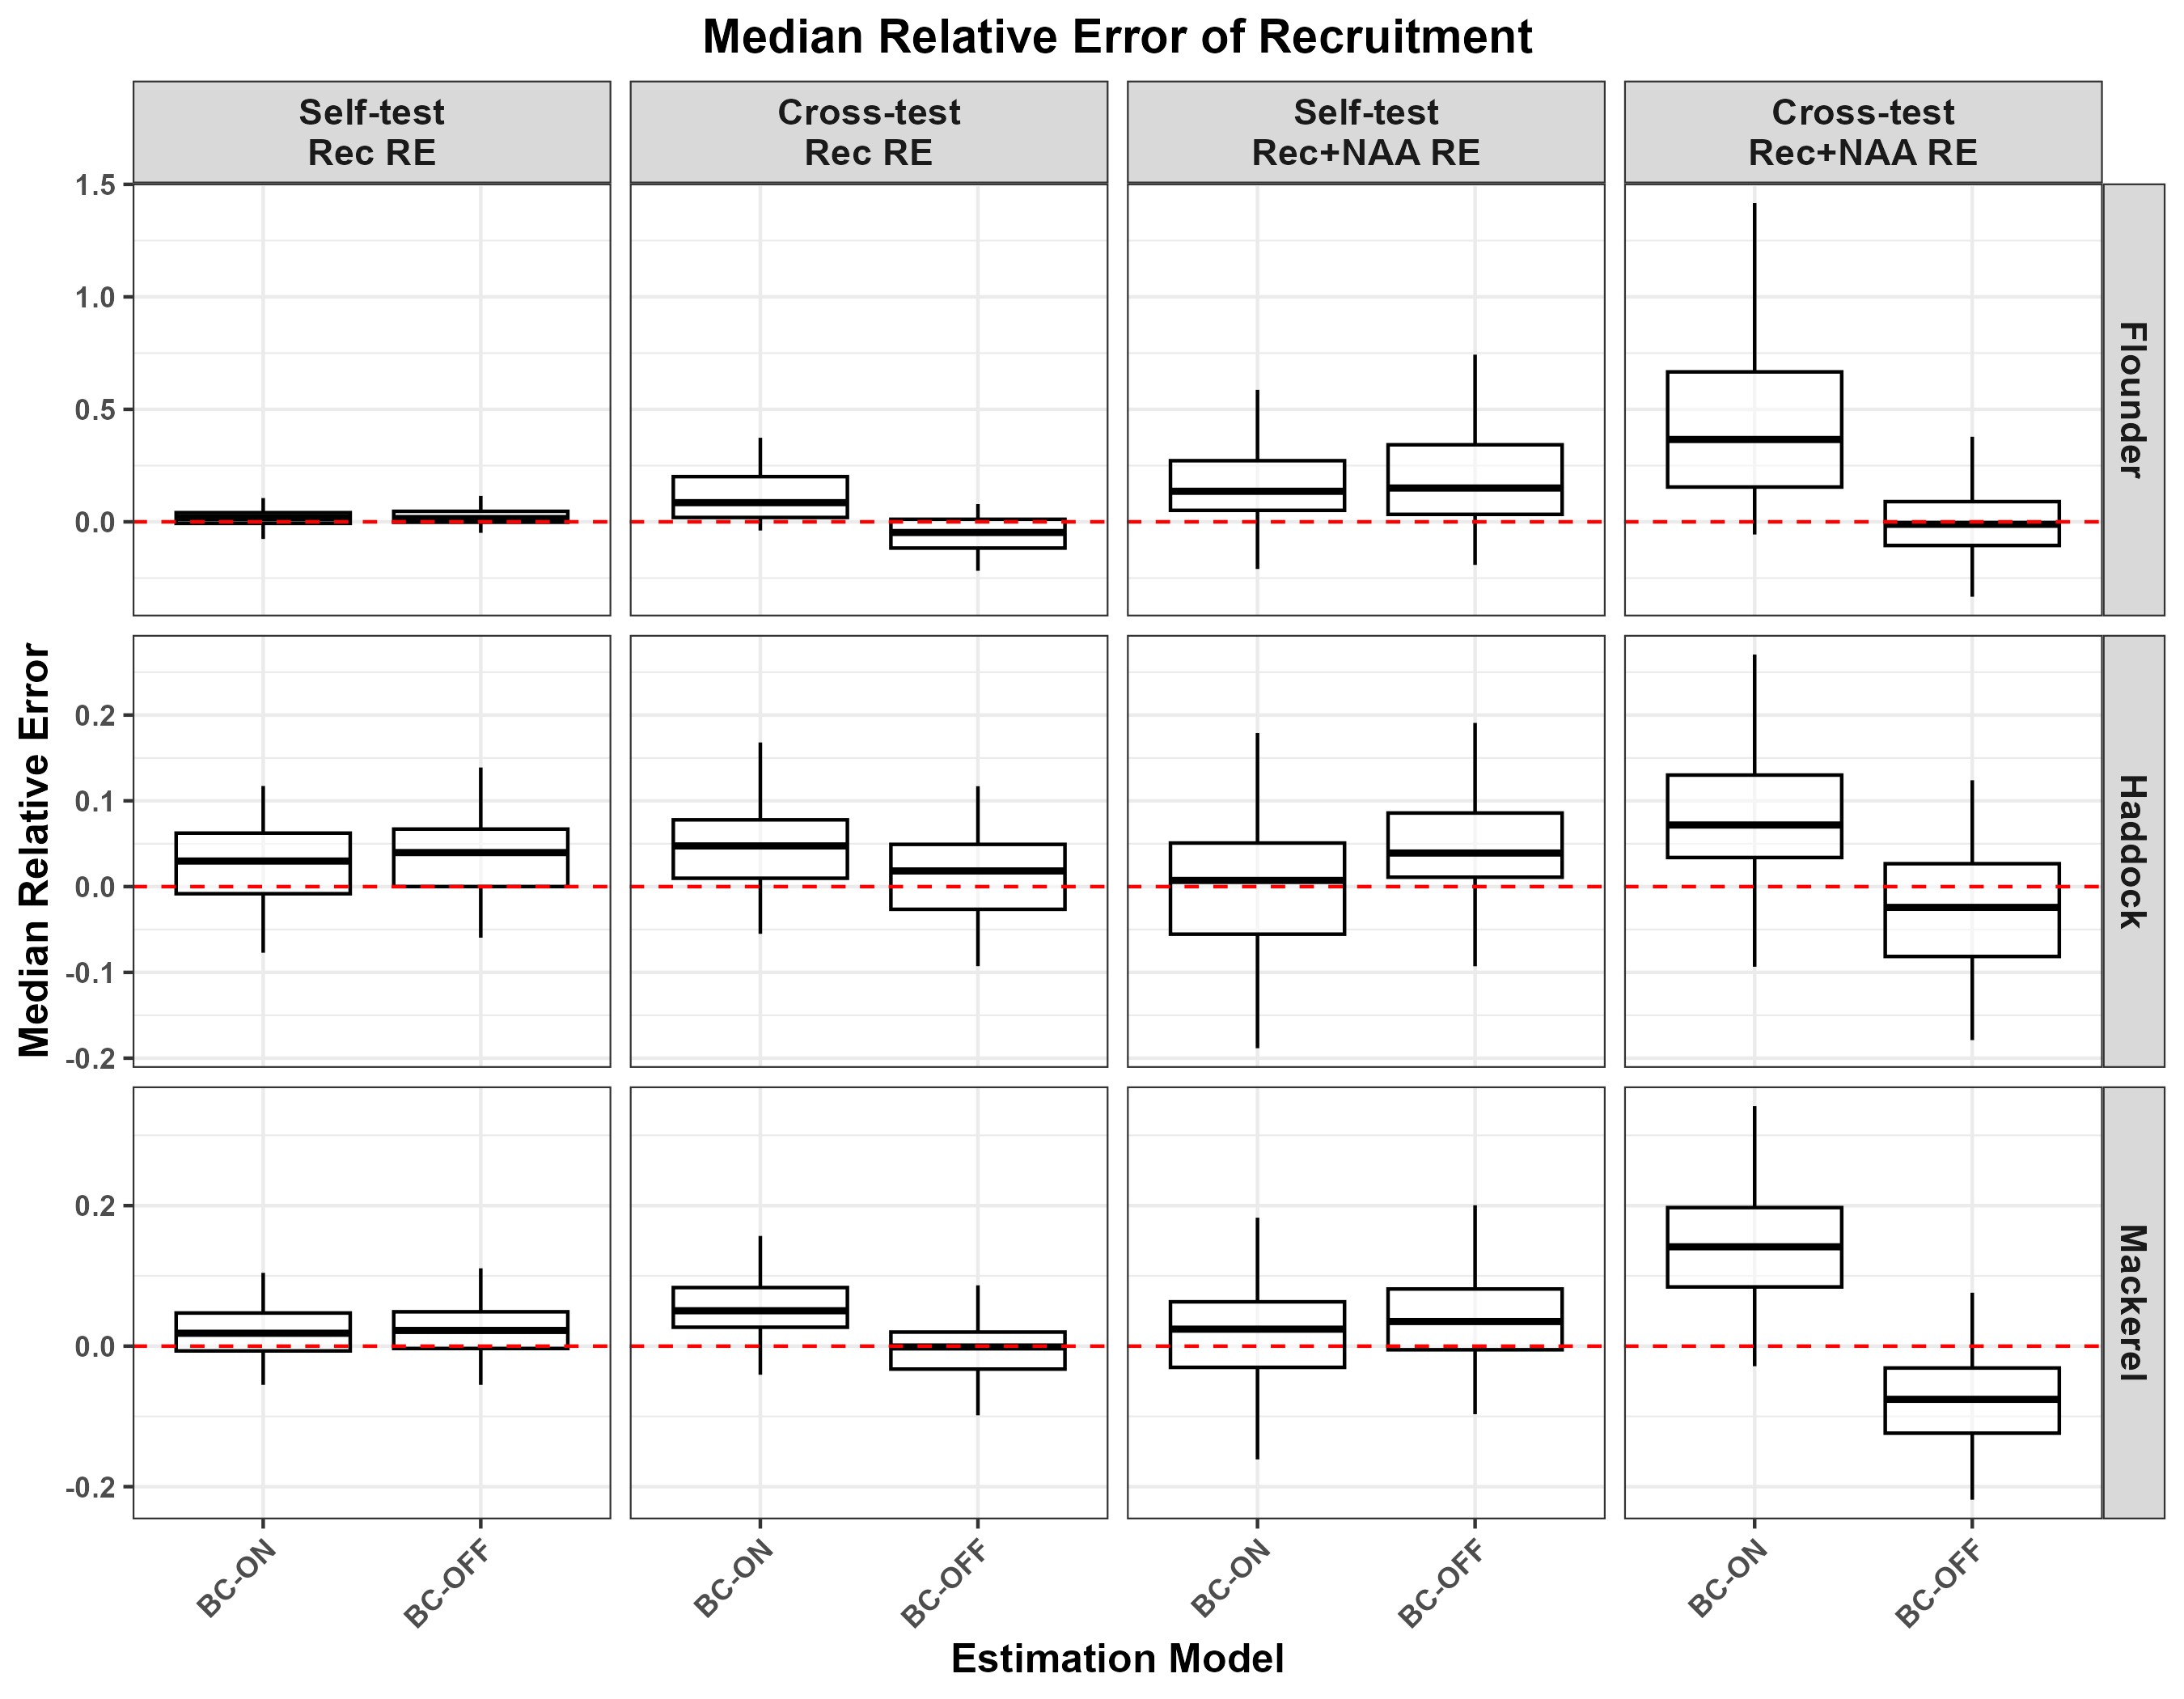
\includegraphics[width=\textwidth]{Revised_Figures&Tables/Median_Rec.PNG}
\caption{Median relative error of recruitment calculated for self-tests and cross-tests. ``Rec RE'' and ``Rec+NAA RE'' in the top facet indicate operating models (OMs) with only recruitment random effects and both recruitment and $NAA$ random effects, respectively.}
\label{fig:Median_Rec}
\end{figure}

\begin{figure}[H]
\centering
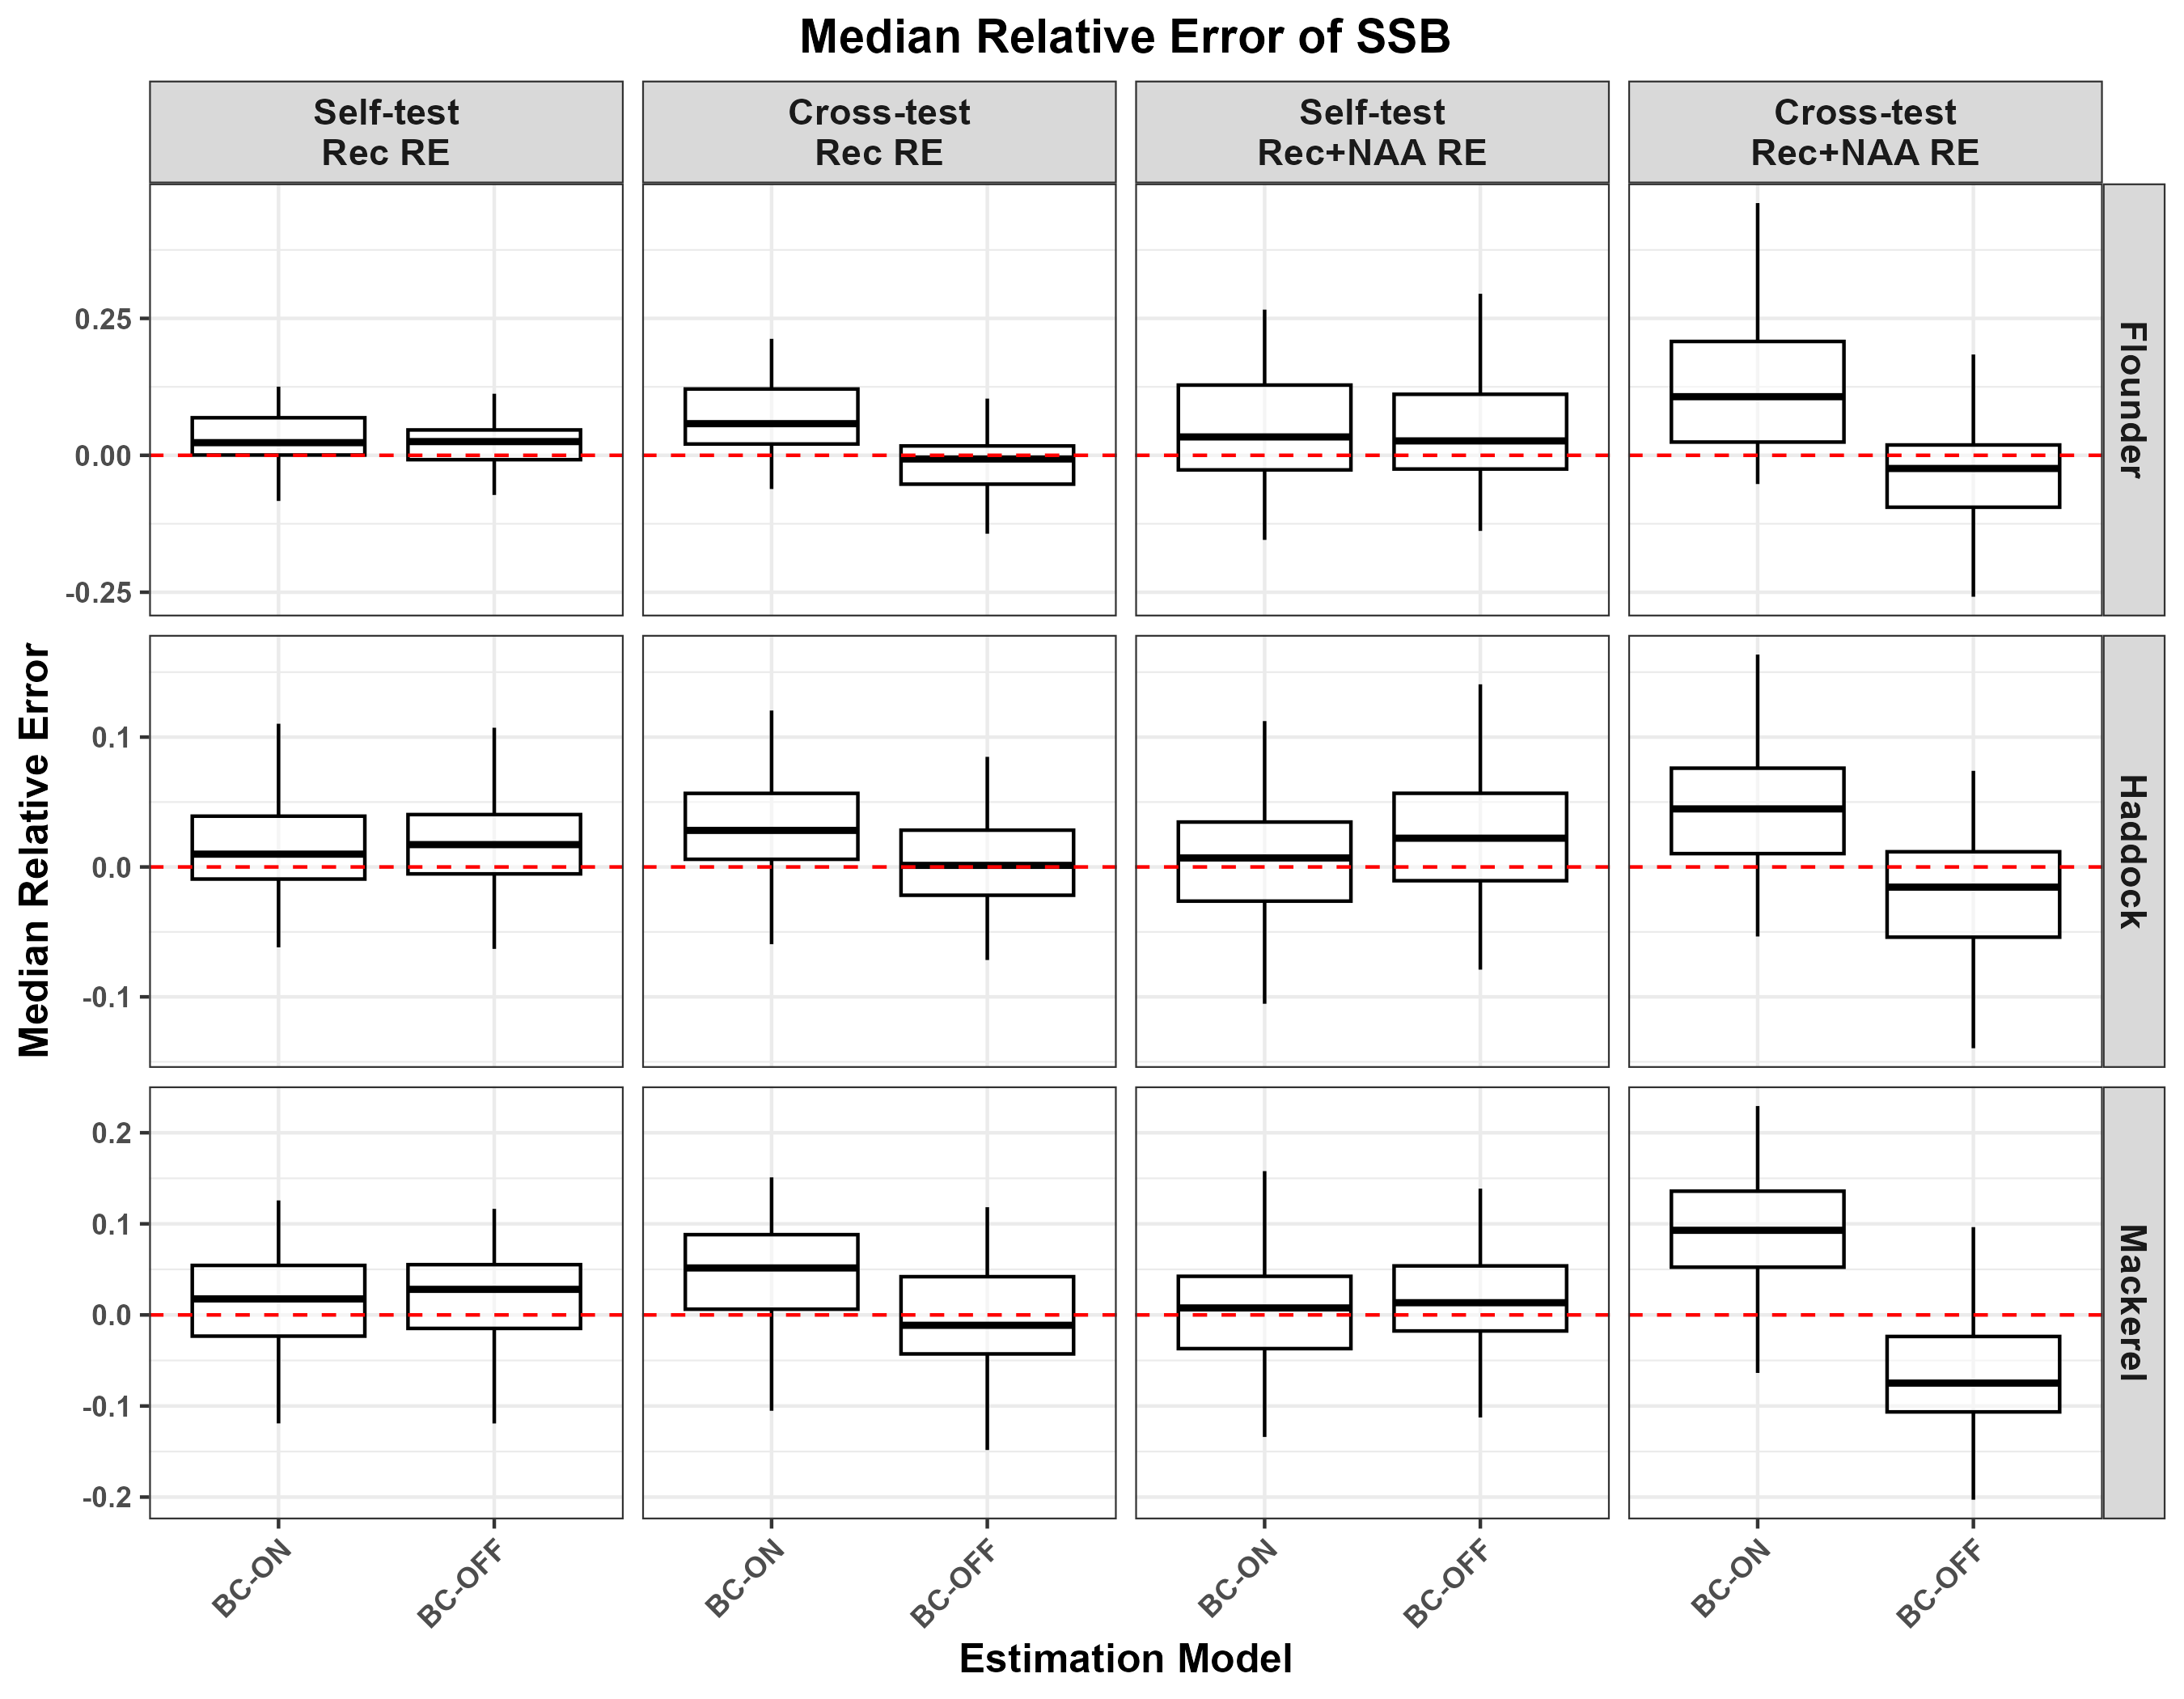
\includegraphics[width=\textwidth]{Revised_Figures&Tables/Median_SSB.PNG}
\caption{Median relative error of $SSB$ calculated for self-tests and cross-tests. ``Rec RE'' and ``Rec+NAA RE'' in the top facet indicate operating models (OMs) with only recruitment random effects and both recruitment and $NAA$ random effects, respectively.}
\label{fig:Median_SSB}
\end{figure}

\begin{figure}[H]
\centering
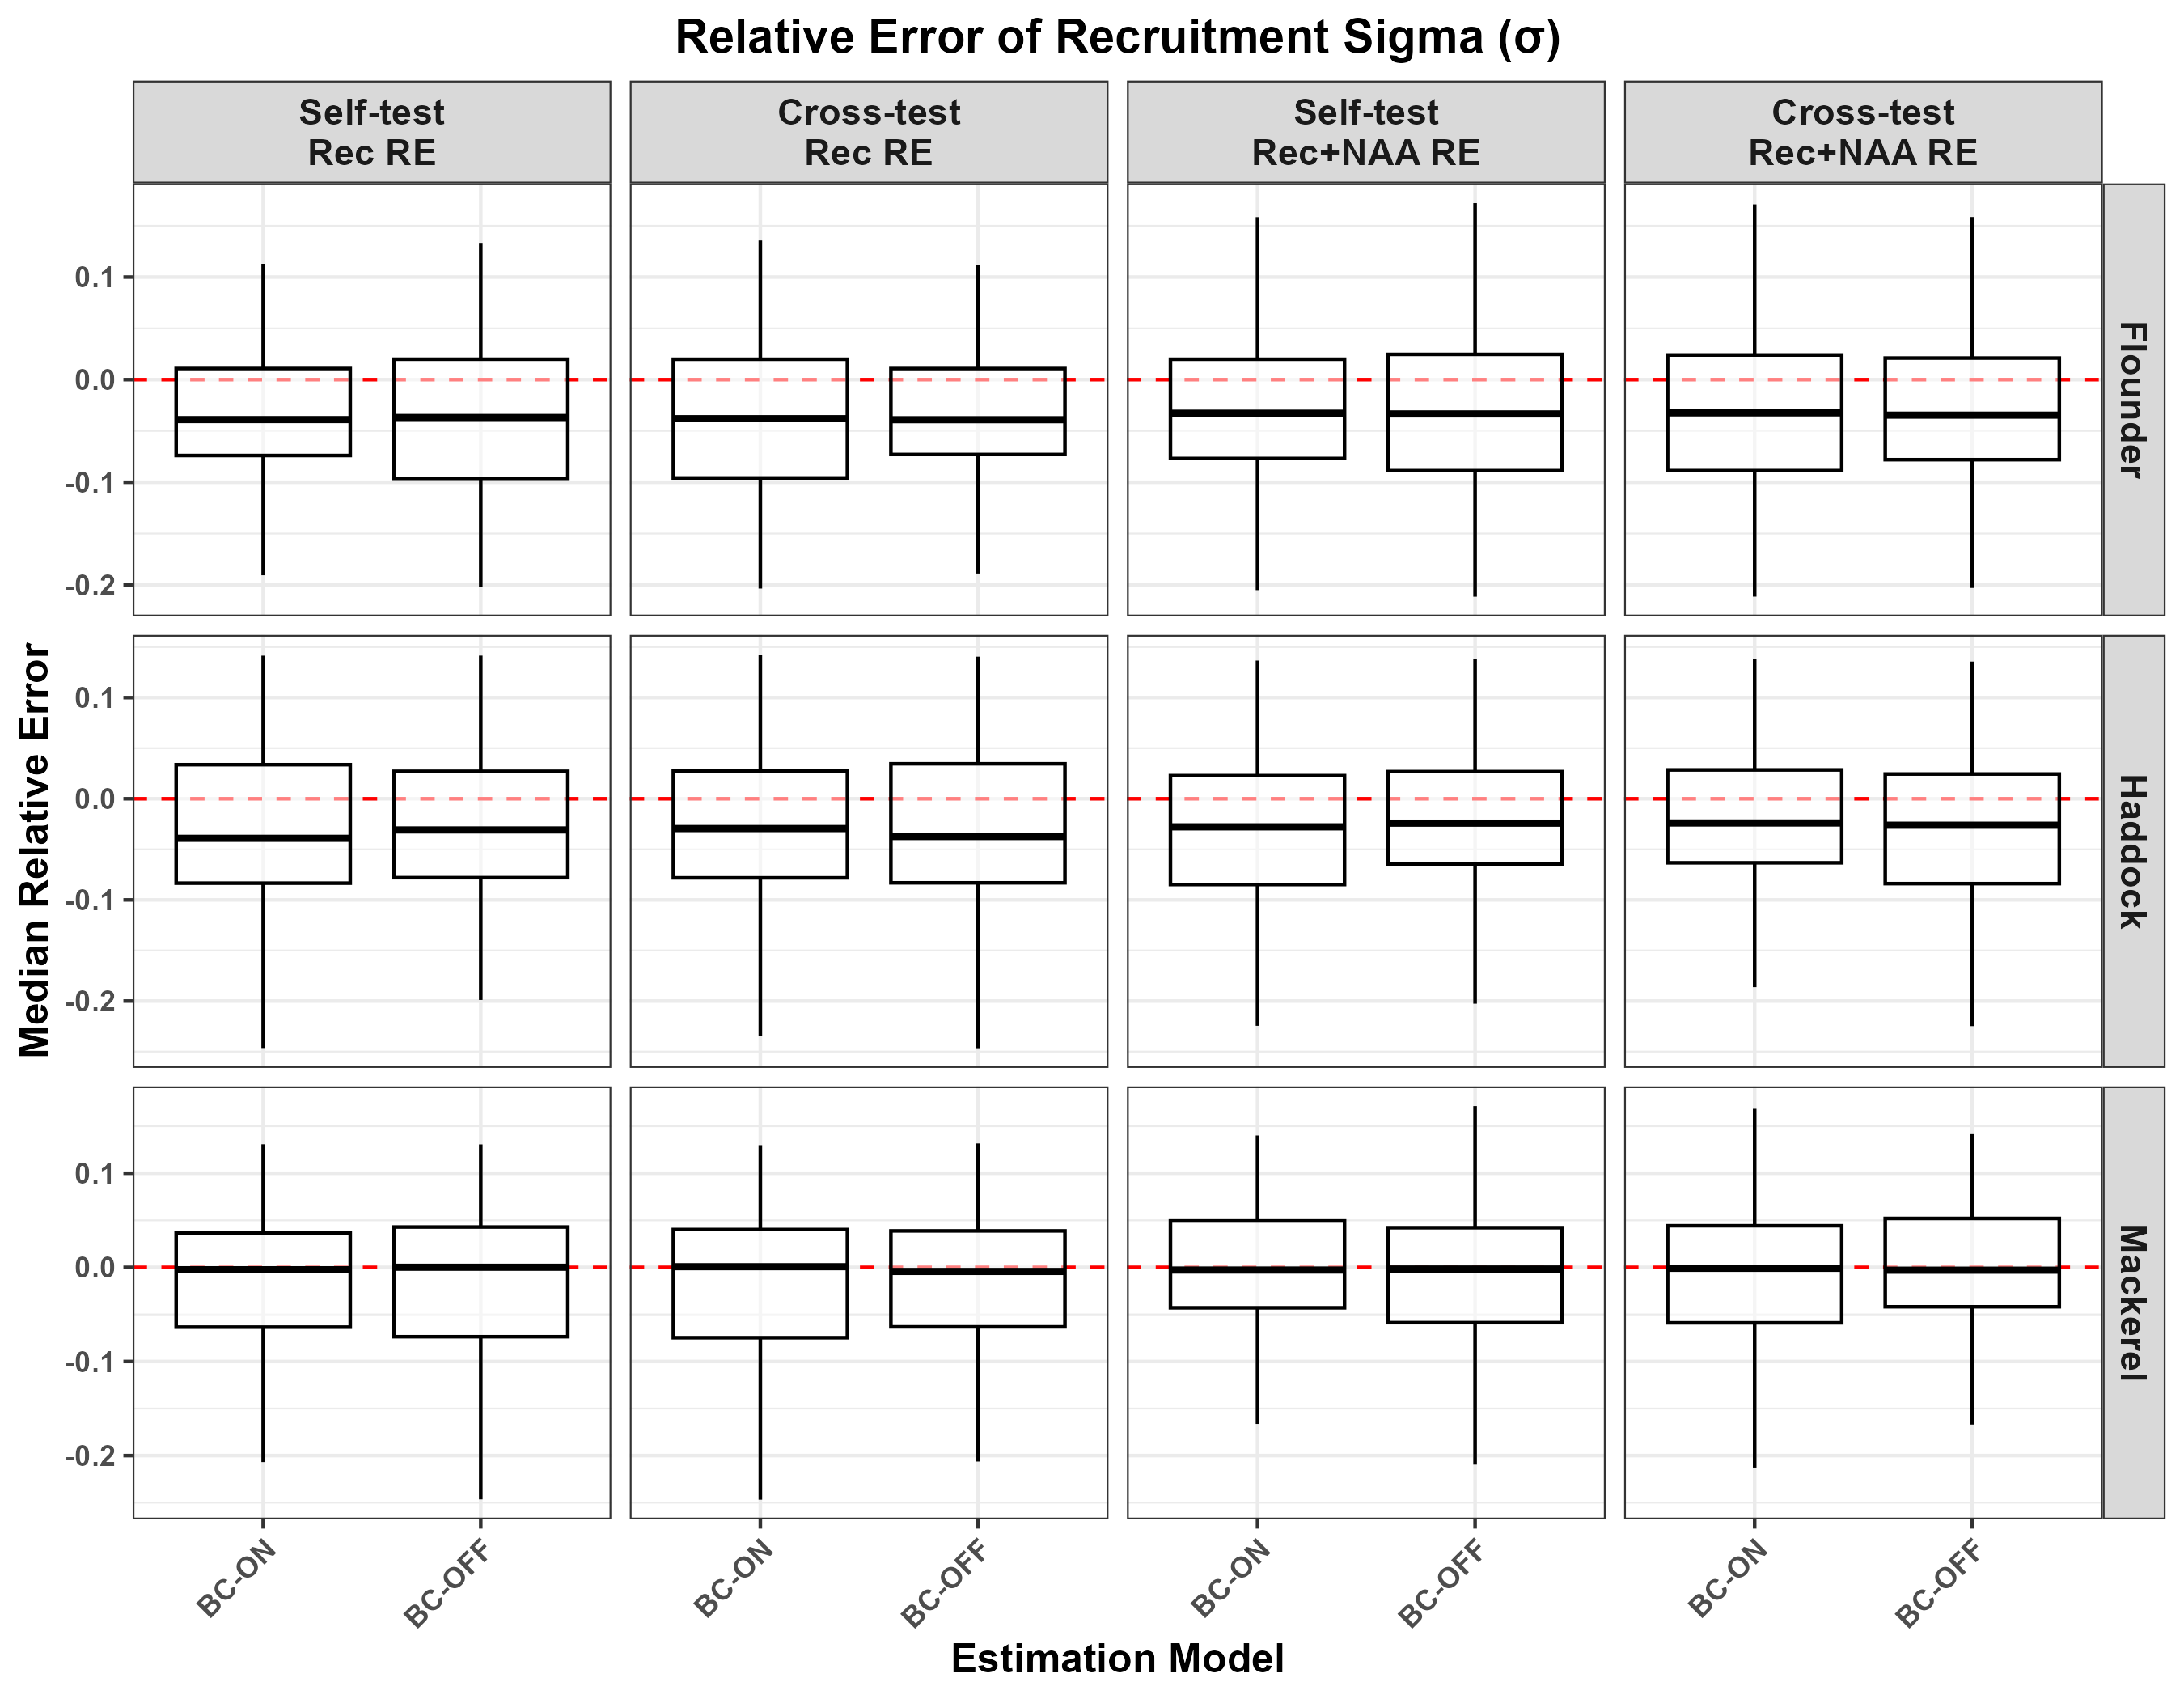
\includegraphics[width=\textwidth]{Revised_Figures&Tables/Rec_sigma.PNG}
\caption{Relative error of recruitment standard deviation ($\sigma_{Rec}$) calculated for self-tests and cross-tests. ``Rec RE'' and ``Rec+NAA RE'' in the top facet indicate operating models (OMs) with only recruitment random effects and both recruitment and $NAA$ random effects, respectively.}
\label{fig:Rec_sigma}
\end{figure}

\begin{figure}[H]
\centering
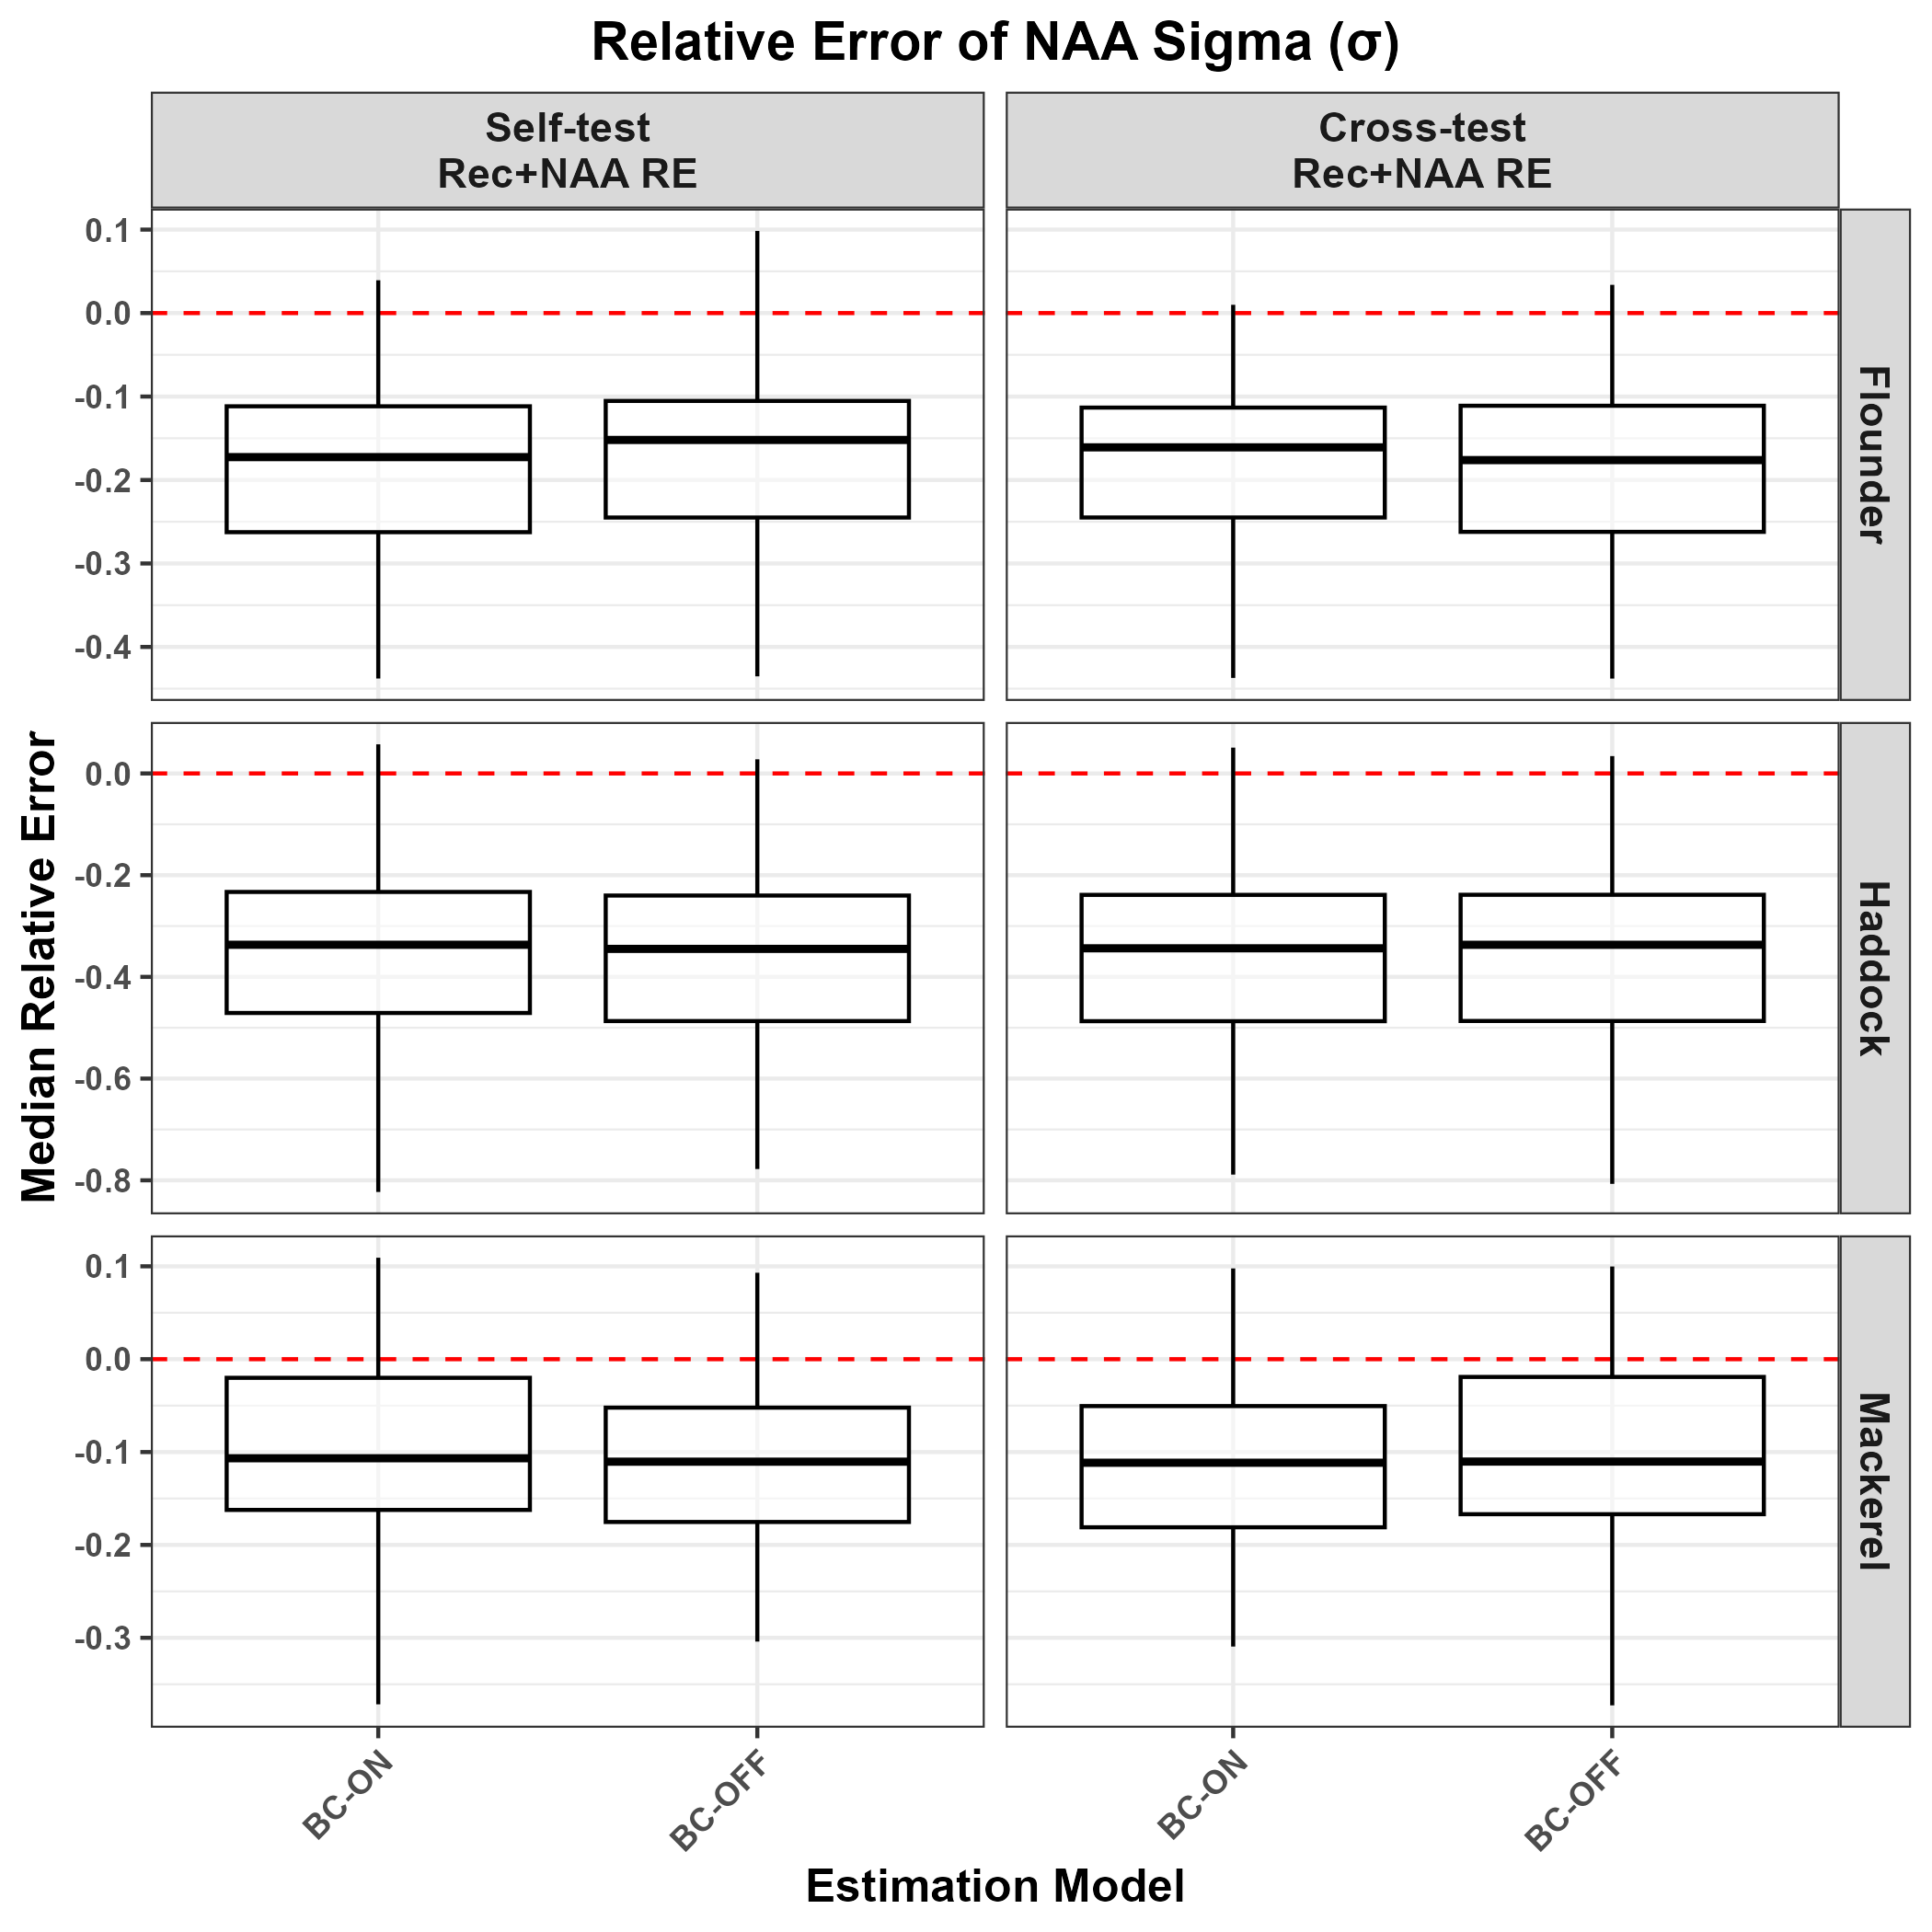
\includegraphics[width=\textwidth]{Revised_Figures&Tables/NAA_sigma.PNG}
\caption{Relative error of $NAA$ standard deviation ($\sigma_{NAA}$) calculated for self-tests and cross-tests. ``Rec RE'' and ``Rec+NAA RE'' in the top facet indicate operating models (OMs) with only recruitment random effects and both recruitment and $NAA$ random effects, respectively.}
\label{fig:NAA_sigma}
\end{figure}

\begin{figure}[H]
\centering
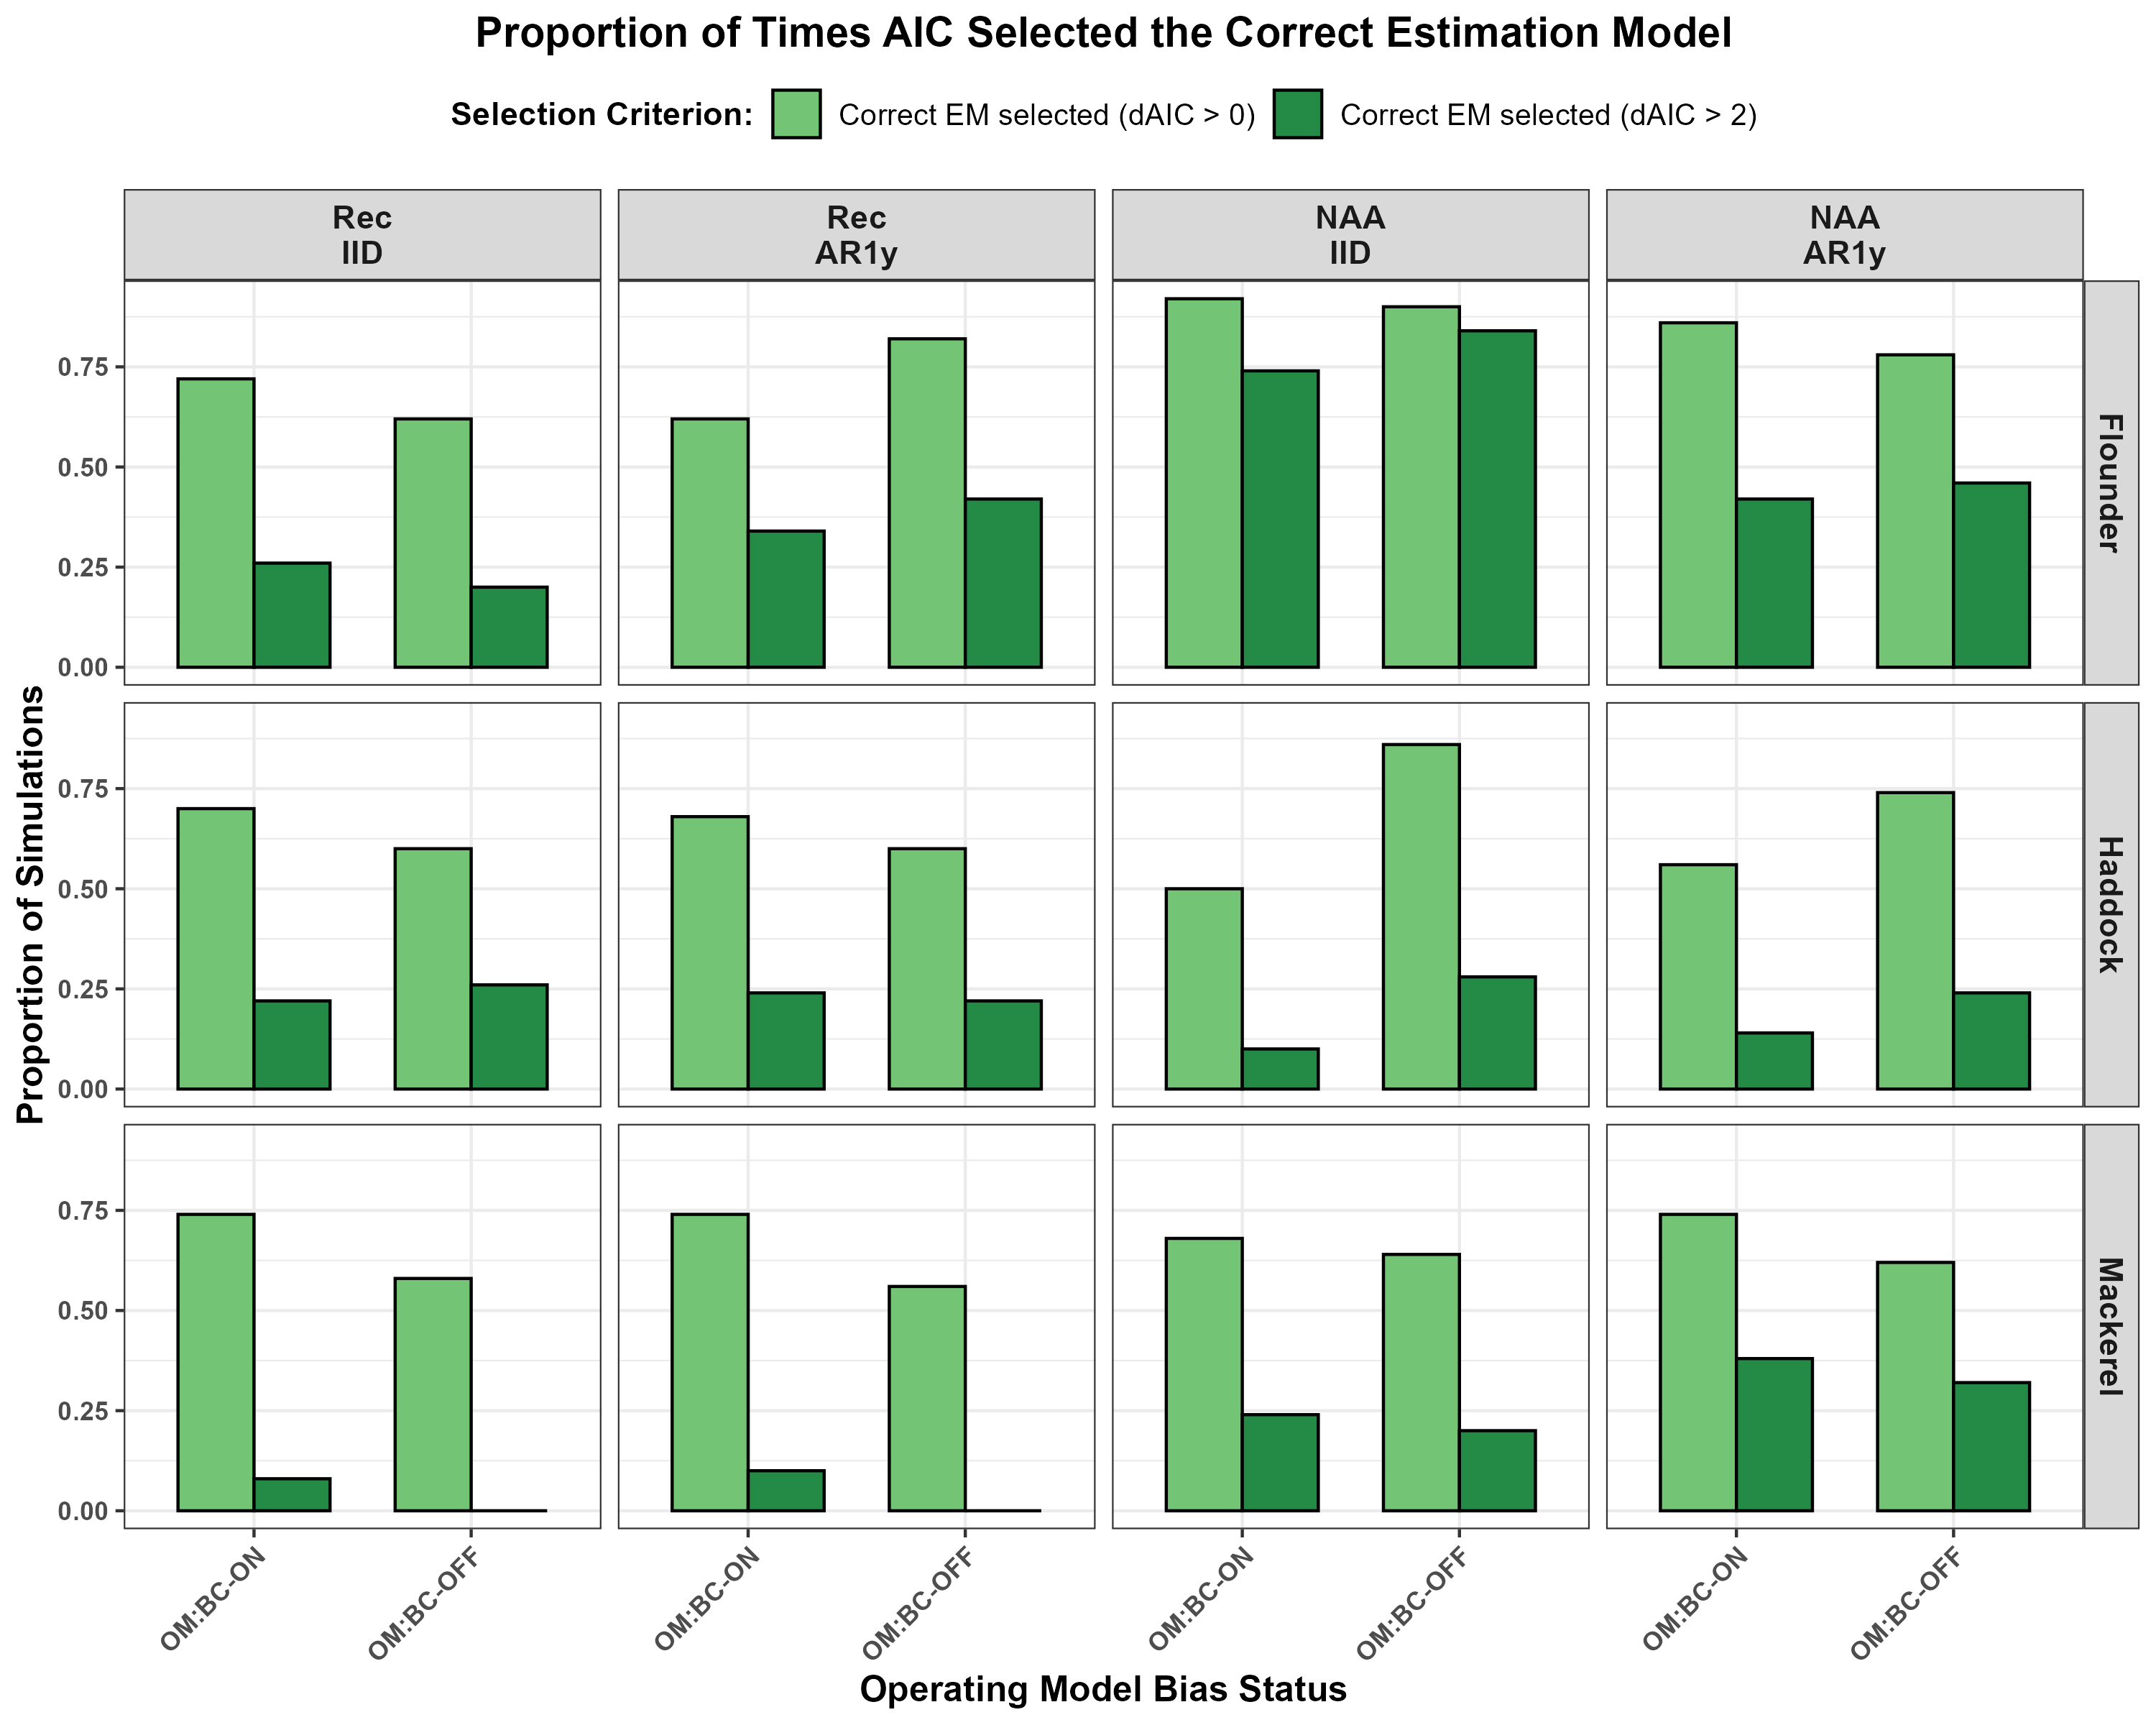
\includegraphics[width=\textwidth]{Revised_Figures&Tables/AIC_select.PNG}
\caption{Proportion of AIC selecting the correct estimation model (EM). Dark green bars represent the proportion of the correct EM selected when the difference in AIC (dAIC) is greater than 2, while light green bars represent the proportion of the correct EM selected when the correct EM has the lowest AIC (dAIC $>0$). The top facet displays operating models (OMs) with different forms of random-effects processes.}
\label{fig:AIC_select}
\end{figure}

\pagebreak

\bibliography{paper}

\pagebreak

\end{document}
